\subsection*{Overview}

%%%Insert this to get the typewriter font so it looks like a real movie script
{\ttfamily
\fontdimen2\font=0.4em
\fontdimen3\font=0.2em
\fontdimen4\font=0.1em
\fontdimen7\font=0.1em
\hyphenchar\font=`\-


%%%%put a hypertarget around the opening bit of text
\hypertarget{scripts_gram_schmidt_and_orthogonal_complements_theory}{This} video depicts the ideas of a subspace sum, a direct sum and an orthogonal complement in ${\mathbb R}^3$.
Firstly, lets start with the subspace sum. Remember that even if $U$ and $V$ are subspaces, their union $U\cup V$ is usually not a subspace. However, the span of their union certainly is
and is called the subspace sum
$$
U+V=\mbox{span}(U\cup V)\, .
$$ 
You need to be aware that this is a sum of vector spaces (not vectors). A picture of this is a pair of planes in ${\mathbb R}^3$: 
 \begin{center}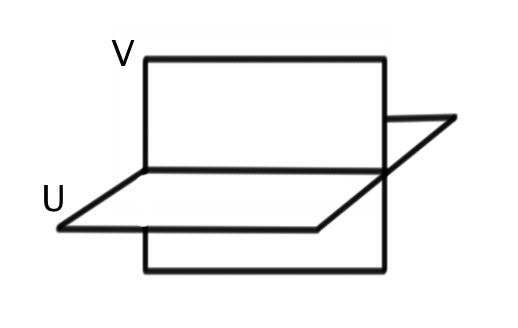
\includegraphics[scale=.3]{\gramSchmidtPath/U+V.jpg}\end{center}
Here $U+V={\mathbb R}^3$. 

Next lets consider a direct sum. This is just the subspace sum for the case when $U\cap V=\{0\}$. For that we can keep the plane $U$
but must replace $V$ by a line:
 \begin{center}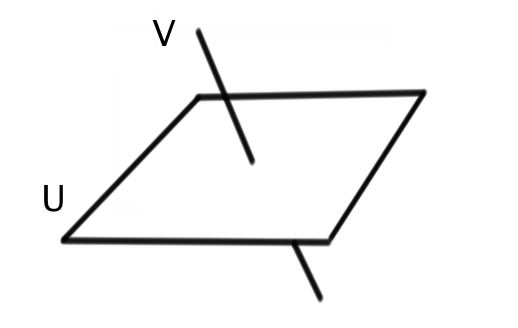
\includegraphics[scale=.3]{\gramSchmidtPath/Uo+V.jpg}\end{center}
 Taking a direct sum we again get the whole space,~$U\oplus V={\mathbb R}^3$. 
 
Now we come to an orthogonal complement. There is not really a notion of subtraction for subspaces but the orthogonal complement comes close. Given $U$
it provides a space $U^\perp$ such that the direct sum returns the whole space:
$$
U\oplus U^\perp = {\mathbb R}^3\, . 
$$
The orthogonal complement $U^\perp$ is the subspace made from all vectors perpendicular to any vector in $U$. Here, we need to just tilt the line $V$ above until it hits $U$ at a right angle:
 \begin{center}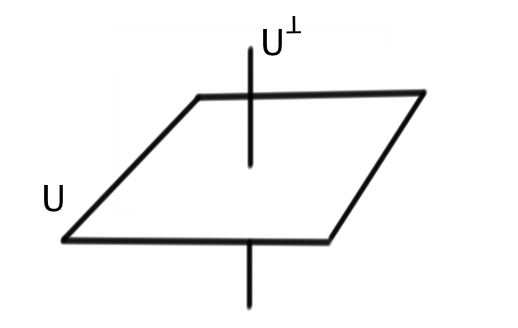
\includegraphics[scale=.3]{\gramSchmidtPath/U+Ut.jpg}\end{center} 
Notice, we can apply the same operation to $U^\perp$ and just get $U$ back again, {\it i.e.}
$$
\big(U^\perp\big)^\perp=U\, .
$$

 
%%%%don't forget to close the bracket so the stuff after your file doesn't look like a movie!
}

%\newpage